\documentclass[10pt,onecolumn,letterpaper]{article}

\usepackage{cvpr}
\usepackage{times}
\usepackage{epsfig}
\usepackage{graphicx}
\usepackage{amsmath}
\usepackage{amssymb}
\usepackage{subfigure}
\usepackage{upgreek}
\usepackage{multirow}
\usepackage{color}

% Include other packages here, before hyperref.

% If you comment hyperref and then uncomment it, you should delete
% egpaper.aux before re-running latex.  (Or just hit 'q' on the first latex
% run, let it finish, and you should be clear).
\usepackage[pagebackref=true,breaklinks=true,letterpaper=true,colorlinks,bookmarks=false]{hyperref}

% \cvprfinalcopy % *** Uncomment this line for the final submission

\def\cvprPaperID{1047} % *** Enter the CVPR Paper ID here
\def\httilde{\mbox{\tt\raisebox{-.5ex}{\symbol{126}}}}

% Pages are numbered in submission mode, and unnumbered in camera-ready
\ifcvprfinal\pagestyle{empty}\fi


\begin{document}

%%%%%%%%% TITLE
\title{Supplementary Material to ``External Prior Guided Internal Prior Learning for Real Noisy Image Denoising"}

\author{First Author\\
Institution1\\
Institution1 address\\
{\tt\small firstauthor@i1.org}
% For a paper whose authors are all at the same institution,
% omit the following lines up until the closing ``}''.
% Additional authors and addresses can be added with ``\and'',
% just like the second author.
% To save space, use either the email address or home page, not both
\and
Second Author\\
Institution2\\
First line of institution2 address\\
{\tt\small secondauthor@i2.org}
}

\maketitle


%%%%%%%%% BODY TEXT
In this supplementary material, we provide:\vspace{-0.1in}
\begin{enumerate}
\item The closed-form solution of the proposed weighted sparse coding model in the main paper.
\vspace{-0.1in}
\item More denoising results on the real noisy images (with no ``ground truth") provided in the dataset \cite{ncwebsite}.
\vspace{-0.1in}
\item More denoising results on the 15 smaller real noisy images (with ``ground truth") used in the dataset \cite{crosschannel2016}.
\vspace{-0.1in}
\item More denoising results on the 60 real noisy images (with ``ground truth") cropped from \cite{crosschannel2016}.
\end{enumerate}
\section{Closed-Form Solution of the Weighted Sparse Coding Problem}
The weighted sparse coding problem in the main paper is:
\begin{equation}\label{equ1}
\setlength{\abovedisplayskip}{1pt}
\setlength{\belowdisplayskip}{1pt}
\min_{\boldsymbol{\alpha}}\|\mathbf{y}-\mathbf{D}\boldsymbol{\alpha}\|_{2}^{2}+\|\mathbf{w}^{T}\boldsymbol{\alpha}\|_{1}.
\end{equation}
Since $\mathbf{D}$ is an orthonormal matrix, problem (\ref{equ1}) is equivalent to 
\begin{equation}\label{equ2}
\setlength{\abovedisplayskip}{1pt}
\setlength{\belowdisplayskip}{1pt}
\min_{\boldsymbol{\alpha}}\|\mathbf{D}^{T}\mathbf{y}-\boldsymbol{\alpha}\|_{2}^{2}+\|\mathbf{w}^{T}\boldsymbol{\alpha}\|_{1}.
\end{equation}
For simplicity, we denote $\mathbf{z} = \mathbf{D^{T}y}$. Since $\mathbf{w}_{i}=c*2\sqrt{2}\sigma^{2}/(\mathbf{\Lambda}_{i}+\varepsilon)$ is positive (please refer to Eq. (18) in the main paper), problem (\ref{equ2}) can be written as
\begin{equation}\label{equ3}
\setlength{\abovedisplayskip}{0.01pt}
\setlength{\belowdisplayskip}{0.01pt}
\min_{\boldsymbol{\alpha}}\sum_{i=1}^{p^{2}}((\mathbf{z}_{i}-\boldsymbol{\alpha}_{i})^{2}+\mathbf{w}_{i}|\boldsymbol{\alpha}_{i}|).
\end{equation}
The problem (\ref{equ3}) is separable w.r.t. $\boldsymbol{\alpha}_{i}$ and can be simplified to $p^{2}$ scalar minimization problems
\begin{equation}\label{equ4}
\setlength{\abovedisplayskip}{2pt}
\setlength{\belowdisplayskip}{1pt}
\min_{\boldsymbol{\alpha}_{i}}(\mathbf{z}_{i}-\boldsymbol{\alpha}_{i})^{2}+\mathbf{w}_{i}|\boldsymbol{\alpha}_{i}|,
\end{equation}
where $i=1,...,p^{2}$. Taking derivative of $\boldsymbol{\alpha}_{i}$ in problem (\ref{equ4}) and setting the derivative to be zero. There are two cases for the solution.

(a) If $\boldsymbol{\alpha}_{i}\ge 0$, we have
\begin{equation}\label{equ5}
\setlength{\abovedisplayskip}{0.1pt}
\setlength{\belowdisplayskip}{0.11pt}
2(\boldsymbol{\alpha}_{i}-\mathbf{z}_{i})+\mathbf{w}_{i}=0.
\end{equation}
\qquad\ \  The solution is
\begin{equation}\label{equ6}
\setlength{\abovedisplayskip}{0.1pt}
\setlength{\belowdisplayskip}{0.1pt}
\hat{\boldsymbol{\alpha}}_{i}=\mathbf{z}_{i}-\frac{\mathbf{w}_{i}}{2} \ge 0.
\end{equation}
\qquad\ \  So $\mathbf{z}_{i}\ge\frac{\mathbf{w}_{i}}{2}> 0$, and the solution $\hat{\boldsymbol{\alpha}}_{i}$ can be written as
\begin{equation}\label{equ7}
\setlength{\abovedisplayskip}{0.1pt}
\setlength{\belowdisplayskip}{0.1pt}
\hat{\boldsymbol{\alpha}}_{i}=\text{sgn}(\mathbf{z}_{i})*(|\mathbf{z}_{i}|-\frac{\mathbf{w}_{i}}{2}),
\end{equation}
\qquad\ \  where $\text{sgn}(\bullet)$ is the sign function. 

(b) If $\boldsymbol{\alpha}_{i}< 0$, we have
\begin{equation}\label{equ8}
\setlength{\abovedisplayskip}{0.1pt}
\setlength{\belowdisplayskip}{0.1pt}
2(\boldsymbol{\alpha}_{i}-\mathbf{z}_{i})-\mathbf{w}_{i}=0.
\end{equation}
\qquad\ \  The solution is
\begin{equation}\label{equ9}
\setlength{\abovedisplayskip}{0.1pt}
\setlength{\belowdisplayskip}{0.1pt}
\hat{\boldsymbol{\alpha}}_{i}=\mathbf{z}_{i}+\frac{\mathbf{w}_{i}}{2} < 0.
\end{equation}
\qquad\ \  So $\mathbf{z}_{i}<-\frac{\mathbf{w}_{i}}{2}< 0$, and the solution $\hat{\boldsymbol{\alpha}}_{i}$ can be written as
\begin{equation}\label{equ10}
\setlength{\abovedisplayskip}{1pt}
\setlength{\belowdisplayskip}{1pt}
\hat{\boldsymbol{\alpha}}_{i}=\text{sgn}(\mathbf{z}_{i})*(-\mathbf{z}_{i}-\frac{\mathbf{w}_{i}}{2})=\text{sgn}(\mathbf{z}_{i})*(|\mathbf{z}_{i}|-\frac{\mathbf{w}_{i}}{2}).
\end{equation} 

In summary, we have the final solution of the weighted sparse coding problem (\ref{equ1}) as
\begin{equation}\label{equ11}
\setlength{\abovedisplayskip}{3pt}
\setlength{\belowdisplayskip}{3pt}
\hat{\boldsymbol{\alpha}}= \text{sgn}(\mathbf{D^{T}y})\odot \text{max}(|\mathbf{D^{T}y}|-\mathbf{w}/2,0),
\end{equation}
where $\odot$ means element-wise multiplication and $|\mathbf{D^{T}y}|$ is the absolute value of each entry of the vector $\mathbf{D^{T}y}$.


\section{More Results on Dataset \cite{ncwebsite}}
In this section, we give more visual comparisons of the competing methods on the real noisy images provided in \cite{ncwebsite}. As can be seen from Figures \ref{fig1}-\ref{fig4}, our proposed method is much better than the state-of-the-art denoising methods. This validates the effectiveness of our proposed external prior guided internal prior learning framework for real noisy image denoising.


\begin{figure}
\centering
\subfigure{
\begin{minipage}[t]{0.244\textwidth}
\centering
\raisebox{-0.15cm}{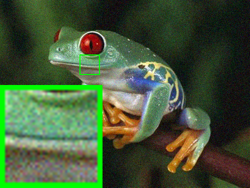
\includegraphics[width=1\textwidth]{imagessupp/resize_frog_noisy.png}}
{\footnotesize (a) Noisy \cite{ncwebsite}   }
\end{minipage}
\begin{minipage}[t]{0.244\textwidth}
\centering
\raisebox{-0.15cm}{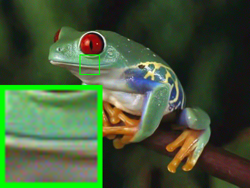
\includegraphics[width=1\textwidth]{imagessupp/resize_frog_cbm3d.png}}
{\footnotesize (b) CBM3D \cite{bm3d,cbm3d}  }
\end{minipage}
\begin{minipage}[t]{0.244\textwidth}
\centering
\raisebox{-0.15cm}{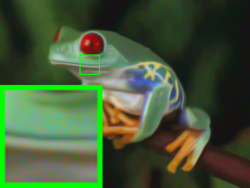
\includegraphics[width=1\textwidth]{imagessupp/resize_frog_wnnm.png}}
{\footnotesize (c) WNNM \cite{wnnm}   }
\end{minipage}
\begin{minipage}[t]{0.244\textwidth}
\centering
\raisebox{-0.15cm}{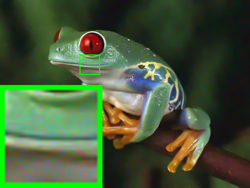
\includegraphics[width=1\textwidth]{imagessupp/resize_frog_mlp.png}}
{\footnotesize (d) MLP \cite{mlp}  }
\end{minipage}
}\vspace{-2mm}
\subfigure{
\begin{minipage}[t]{0.244\textwidth}
\centering
\raisebox{-0.15cm}{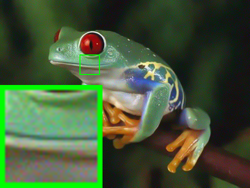
\includegraphics[width=1\textwidth]{imagessupp/resize_frog_tnrd.png}}
{\footnotesize (e) TNRD \cite{chen2015learning}}
\end{minipage}
\begin{minipage}[t]{0.244\textwidth}
\centering
\raisebox{-0.15cm}{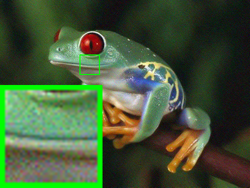
\includegraphics[width=1\textwidth]{imagessupp/resize_frog_ni.png}}
{\footnotesize (f) NI \cite{neatimage}  }
\end{minipage}
\begin{minipage}[t]{0.244\textwidth}
\centering
\raisebox{-0.15cm}{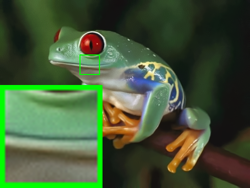
\includegraphics[width=1\textwidth]{imagessupp/resize_frog_nc.png}}
{\footnotesize (g) NC \cite{noiseclinic,ncwebsite}   }
\end{minipage}
\begin{minipage}[t]{0.244\textwidth}
\centering
\raisebox{-0.15cm}{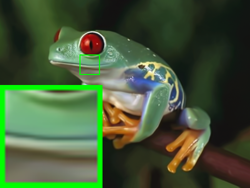
\includegraphics[width=1\textwidth]{imagessupp/resize_frog_ours.png}}
{\footnotesize (h) Ours  }
\end{minipage}
}
\vspace{-2mm}
\caption{Denoised images of the real noisy image ``Frog" \cite{ncwebsite} by different methods. The images are better to be zoomed in on screen.}
\label{fig1}
\end{figure}


\begin{figure}\vspace{3mm}
\centering
\subfigure{
\begin{minipage}[t]{0.244\textwidth}
\centering
\raisebox{-0.15cm}{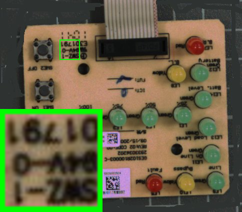
\includegraphics[width=1\textwidth]{imagessupp/resize_br_Noisy_circuit.png}}
{\footnotesize (a) Noisy \cite{ncwebsite}   }
\end{minipage}
\begin{minipage}[t]{0.244\textwidth}
\centering
\raisebox{-0.15cm}{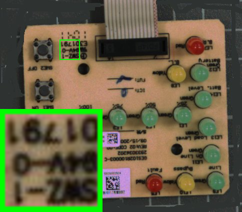
\includegraphics[width=1\textwidth]{imagessupp/resize_br_BM3D_circuit.png}}
{\footnotesize (b) CBM3D \cite{bm3d,cbm3d}  }
\end{minipage}
\begin{minipage}[t]{0.244\textwidth}
\centering
\raisebox{-0.15cm}{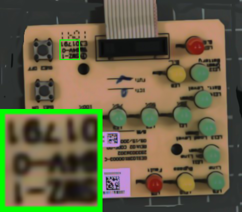
\includegraphics[width=1\textwidth]{imagessupp/resize_br_WNNM_circuit.png}}
{\footnotesize (c) WNNM \cite{wnnm}   }
\end{minipage}
\begin{minipage}[t]{0.244\textwidth}
\centering
\raisebox{-0.15cm}{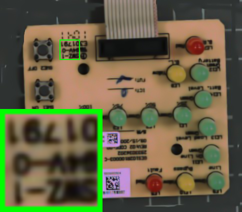
\includegraphics[width=1\textwidth]{imagessupp/resize_br_MLP_circuit.png}}
{\footnotesize (d) MLP \cite{mlp}  }
\end{minipage}
}\vspace{-2mm}
\subfigure{
\begin{minipage}[t]{0.244\textwidth}
\centering
\raisebox{-0.15cm}{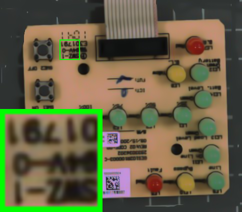
\includegraphics[width=1\textwidth]{imagessupp/resize_br_TRD_circuit.png}}
{\footnotesize (e) TNRD \cite{chen2015learning}}
\end{minipage}
\begin{minipage}[t]{0.244\textwidth}
\centering
\raisebox{-0.15cm}{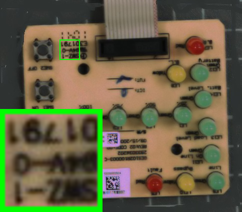
\includegraphics[width=1\textwidth]{imagessupp/resize_br_NI_circuit.png}}
{\footnotesize (f) NI \cite{neatimage}  }
\end{minipage}
\begin{minipage}[t]{0.244\textwidth}
\centering
\raisebox{-0.15cm}{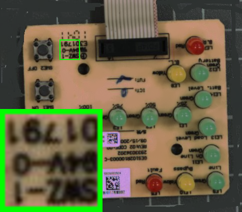
\includegraphics[width=1\textwidth]{imagessupp/resize_br_NC_circuit.png}}
{\footnotesize (g) NC \cite{noiseclinic,ncwebsite}   }
\end{minipage}
\begin{minipage}[t]{0.244\textwidth}
\centering
\raisebox{-0.15cm}{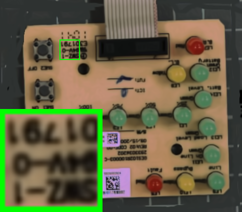
\includegraphics[width=1\textwidth]{imagessupp/resize_br_Guided_circuit.png}}
{\footnotesize (h) Ours  }
\end{minipage}
}
\vspace{-2mm}
\caption{Denoised images of the real noisy image ``Circuit" \cite{ncwebsite} by different methods. The images are better to be zoomed in on screen.}
\label{fig2}
\end{figure}

\begin{figure}\vspace{3mm}
\centering
\subfigure{
\begin{minipage}[t]{0.244\textwidth}
\centering
\raisebox{-0.15cm}{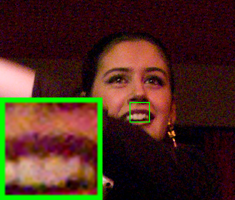
\includegraphics[width=1\textwidth]{imagessupp/resize_br_Noisy_woman.png}}
{\footnotesize (a) Noisy \cite{ncwebsite}   }
\end{minipage}
\begin{minipage}[t]{0.244\textwidth}
\centering
\raisebox{-0.15cm}{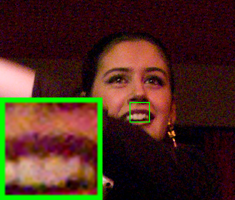
\includegraphics[width=1\textwidth]{imagessupp/resize_br_BM3D_woman.png}}
{\footnotesize (b) CBM3D \cite{bm3d,cbm3d}  }
\end{minipage}
\begin{minipage}[t]{0.244\textwidth}
\centering
\raisebox{-0.15cm}{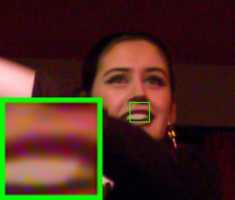
\includegraphics[width=1\textwidth]{imagessupp/resize_br_WNNM_woman.png}}
{\footnotesize (c) WNNM \cite{wnnm}   }
\end{minipage}
\begin{minipage}[t]{0.244\textwidth}
\centering
\raisebox{-0.15cm}{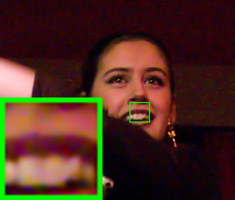
\includegraphics[width=1\textwidth]{imagessupp/resize_br_MLP_woman.png}}
{\footnotesize (d) MLP \cite{mlp}  }
\end{minipage}
}\vspace{-2mm}
\subfigure{
\begin{minipage}[t]{0.244\textwidth}
\centering
\raisebox{-0.15cm}{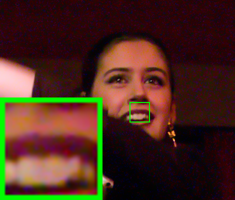
\includegraphics[width=1\textwidth]{imagessupp/resize_br_TRD_woman.png}}
{\footnotesize (e) TNRD \cite{chen2015learning}}
\end{minipage}
\begin{minipage}[t]{0.244\textwidth}
\centering
\raisebox{-0.15cm}{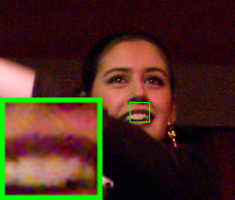
\includegraphics[width=1\textwidth]{imagessupp/resize_br_NI_woman.png}}
{\footnotesize (f) NI \cite{neatimage}  }
\end{minipage}
\begin{minipage}[t]{0.244\textwidth}
\centering
\raisebox{-0.15cm}{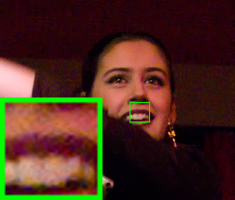
\includegraphics[width=1\textwidth]{imagessupp/resize_br_NC_woman.png}}
{\footnotesize (g) NC \cite{noiseclinic,ncwebsite}   }
\end{minipage}
\begin{minipage}[t]{0.244\textwidth}
\centering
\raisebox{-0.15cm}{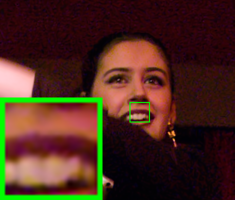
\includegraphics[width=1\textwidth]{imagessupp/resize_br_Guided_woman.png}}
{\footnotesize (h) Ours  }
\end{minipage}
}
\vspace{-2mm}
\caption{Denoised images of the real noisy image ``Woman" \cite{ncwebsite} by different methods. The images are better to be zoomed in on screen.}
\label{fig3}
\end{figure}



{\small
\bibliographystyle{unsrt}
\bibliography{egbib}
}

\end{document}
